\documentclass[12pt]{article}

% ---------------- PAQUETES ----------------
\usepackage[spanish]{babel}
\usepackage[utf8]{inputenc}
\usepackage[T1]{fontenc}
\usepackage{geometry}
\usepackage{graphicx}
\usepackage{listings}
\usepackage{xcolor}
\usepackage{amsmath}
\usepackage{titlesec}

\geometry{a4paper, margin=2.5cm}

% ---------------- CONFIGURACION CODIGO ----------------
\lstset{
    language=Octave,
    basicstyle=\ttfamily\small,
    keywordstyle=\color{blue},
    stringstyle=\color{red},
    commentstyle=\color{green!60!black},
    numbers=left,
    numberstyle=\tiny,
    frame=single,
    breaklines=true
}

% ---------------- FORMATO TITULOS ----------------
\titleformat{\section}
{\large\bfseries}
{\thesection.}{0.5em}{}

\begin{document}

% =====================================================
% CARATULA
% =====================================================

\begin{titlepage}
\centering

{\large UNIVERSIDAD MAYOR DE SAN ANDRES \\}
\vspace{0.3cm}
{\large FACULTAD DE CIENCIAS PURAS Y NATURALES \\}
\vspace{0.3cm}
{\large CARRERA DE MATEMATICA \\}

\vspace{3cm}

{\Huge \textbf{RESOLUCION DE PROBLEMAS}}\\
\vspace{0.3cm}
{\Huge \textbf{MATEMATICOS EN OCTAVE}}

\vspace{2cm}

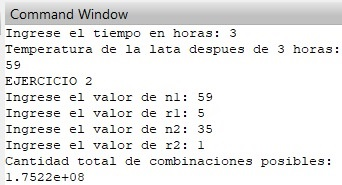
\includegraphics[width=0.25\textwidth]{ejemplo1_2.jpg}

\vspace{2cm}

\begin{flushleft}
\textbf{Materia:} Computacion Cientifica \\[0.3cm]
\textbf{Sigla:} Computacion 117 \\[0.3cm]
\textbf{Docente:} Lic. Brigida \\[0.3cm]
\textbf{Estudiante:} Miguel Rodriguez Achocalla \\[0.3cm]
\end{flushleft}

\vfill

{\large La Paz -- Bolivia \\}
{\large 2026}

\end{titlepage}

% =====================================================
% INDICE
% =====================================================

\tableofcontents
\newpage

% =====================================================
% INTRODUCCION
% =====================================================

\section{Introduccion}

La programacion cientifica permite resolver problemas matematicos mediante algoritmos y herramientas computacionales. En la actualidad, programas como GNU Octave facilitan el desarrollo de calculos numericos y simulaciones de manera sencilla y eficiente.

En el presente informe se desarrollan dos problemas matematicos utilizando Octave. El primero corresponde al modelo de transferencia de calor mediante una ecuacion exponencial, mientras que el segundo aplica la formula de combinaciones para calcular las posibilidades existentes en el juego de loteria Powerball.

El trabajo tiene como finalidad fortalecer el aprendizaje de estructuras basicas de programacion, ingreso de datos y uso de funciones matematicas integradas dentro del entorno Octave.

% =====================================================
% OBJETIVOS
% =====================================================

\section{Objetivos}

\subsection{Objetivo General}

Desarrollar programas en Octave para resolver problemas matematicos relacionados con transferencia de calor y combinaciones.

\subsection{Objetivos Especificos}

\begin{itemize}
\item Aplicar formulas matematicas mediante programacion.
\item Utilizar funciones integradas de Octave.
\item Realizar ingreso de datos por teclado.
\item Mostrar resultados numericos de manera automatica.
\end{itemize}

% =====================================================
% FUNDAMENTO TEORICO
% =====================================================

\section{Fundamento Teorico}

\subsection{Transferencia de calor}

La transferencia de calor describe el comportamiento de la temperatura de un cuerpo cuando es expuesto a un medio con distinta temperatura. Una de las ecuaciones mas utilizadas es:

\[
T = Ts + (T_0 - Ts)e^{-kt}
\]

Donde:

\begin{itemize}
\item $T$ = temperatura final del objeto.
\item $Ts$ = temperatura del medio.
\item $T_0$ = temperatura inicial.
\item $k$ = constante de enfriamiento.
\item $t$ = tiempo.
\end{itemize}

Esta ecuacion representa un modelo exponencial de enfriamiento.

\subsection{Combinaciones}

Las combinaciones permiten calcular cuantas maneras existen de seleccionar elementos de un conjunto sin importar el orden.

La formula utilizada es:

\[
C_{n,r} = \frac{n!}{r!(n-r)!}
\]

Donde:

\begin{itemize}
\item $n$ = cantidad total de elementos.
\item $r$ = cantidad de elementos seleccionados.
\item $!$ = factorial.
\end{itemize}

% =====================================================
% DESARROLLO DE LOS EJERCICIOS
% =====================================================

\section{Desarrollo de los Ejercicios}

\subsection{Ejercicio 1: Transferencia de calor}

Se plantea el problema de una lata de refresco con temperatura inicial de $120^\circ F$ colocada dentro de un refrigerador a $38^\circ F$.

Los datos utilizados fueron:

\begin{itemize}
\item $Ts = 38$
\item $T_0 = 120$
\item $k = 0.45$
\item $t = 3$
\end{itemize}

El resultado obtenido fue:

\[
T = 59^\circ F
\]

\subsection{Ejercicio 2: Combinaciones Powerball}

En este ejercicio se calcularon las posibles combinaciones del juego Powerball utilizando:

\[
C_{59,5} \times C_{35,1}
\]

El resultado obtenido fue aproximadamente:

\[
175090000
\]

combinaciones posibles.

% =====================================================
% CODIGO FUENTE
% =====================================================

\section{Codigo Fuente}

\begin{lstlisting}
% =========================================
% EJERCICIO 1 - TRANSFERENCIA DE CALOR
% =========================================

disp("EJERCICIO 1")

% Ingreso de datos
Ts = input("Ingrese la temperatura del refrigerador: ");
T0 = input("Ingrese la temperatura inicial de la lata: ");
k = input("Ingrese el valor de k: ");
t = input("Ingrese el tiempo en horas: ");

% Formula
T = round(Ts + (T0 - Ts) * exp(-k * t));

% Resultado
disp("Temperatura de la lata despues de 3 horas:")
disp(T)

% =========================================
% EJERCICIO 2 - COMBINACIONES POWERBALL
% =========================================

disp("EJERCICIO 2")

% Ingreso de datos
n1 = input("Ingrese el valor de n1: ");
r1 = input("Ingrese el valor de r1: ");

n2 = input("Ingrese el valor de n2: ");
r2 = input("Ingrese el valor de r2: ");

% Formula de combinaciones
C1 = factorial(n1) / (factorial(r1) * factorial(n1 - r1));
C2 = factorial(n2) / (factorial(r2) * factorial(n2 - r2));

% Total
total = C1 * C2;

% Resultado
disp("Cantidad total de combinaciones posibles:")
disp(total)
\end{lstlisting}

% =====================================================
% EJECUCION
% =====================================================

\section{Ejecucion del Programa}

\begin{figure}[h]
\centering
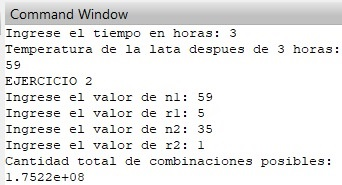
\includegraphics[width=0.9\textwidth]{ejemplo1_2.jpg}
\caption{Ejecucion del programa en GNU Octave}
\end{figure}

% =====================================================
% EXPLICACION
% =====================================================

\section{Explicacion de la Corrida}

El programa inicia solicitando datos mediante la funcion \texttt{input()}. En el primer ejercicio se ingresan valores relacionados con temperatura y tiempo para calcular el enfriamiento de la lata mediante una funcion exponencial.

Posteriormente, en el segundo ejercicio, el usuario introduce valores de combinaciones correspondientes al juego Powerball. El sistema utiliza la funcion integrada \texttt{factorial()} para calcular automaticamente las combinaciones posibles.

Finalmente, el programa muestra los resultados en pantalla utilizando la funcion \texttt{disp()}.

% =====================================================
% VENTAJAS DEL USO DE OCTAVE
% =====================================================

\section{Ventajas del Uso de Octave}

\begin{itemize}
\item Permite realizar calculos matematicos complejos facilmente.
\item Posee funciones matematicas integradas.
\item Facilita la simulacion de problemas cientificos.
\item Es una herramienta gratuita y de codigo abierto.
\item Su sintaxis es sencilla para estudiantes principiantes.
\end{itemize}

% =====================================================
% CONCLUSIONES
% =====================================================

\section{Conclusiones}

Se desarrollaron satisfactoriamente dos ejercicios matematicos utilizando GNU Octave. El primero permitio aplicar un modelo de transferencia de calor mediante una ecuacion exponencial, mientras que el segundo utilizo combinaciones y factoriales para resolver un problema de probabilidad.

El trabajo permitio comprender el uso de variables, funciones matematicas, ingreso de datos y visualizacion de resultados en un entorno de programacion cientifica.

Asimismo, se evidencio que Octave constituye una herramienta importante para la resolucion de problemas matematicos y computacionales.

% =====================================================
% RECOMENDACIONES
% =====================================================

\section{Recomendaciones}

\begin{itemize}
\item Utilizar nombres adecuados para los archivos y evitar conflictos con funciones integradas.
\item Verificar correctamente el ingreso de datos.
\item Implementar validaciones para evitar errores en la ejecucion.
\item Practicar con ejercicios matematicos adicionales para mejorar la logica de programacion.
\end{itemize}

% =====================================================
% BIBLIOGRAFIA
% =====================================================

\section{Bibliografia}

\begin{itemize}
\item Eaton, J. (2022). \textit{GNU Octave Manual}. GNU Project.
\item Kreyszig, E. (2011). \textit{Matematicas Avanzadas para Ingenieria}. Wiley.
\item Stewart, J. (2013). \textit{Calculo de Varias Variables}. Cengage Learning.
\item Documentacion oficial GNU Octave.
\end{itemize}

\end{document}